\section{Strategy-Muster}

\subsection{Problemstellung}
\begin{itemize}
\item Es soll eine Simulation fuer ein Spiel mit diversen Entenarten geschrieben werden.
\item Entenarten besitzen verschiedene Eigenschaften.
\item In manchen Faellen nicht nur verschiedene Auspraegungen, sondern sogar nicht existent. 
\item Verschiedene Arten sollen aber alle von der selben Klasse erben. 
\end{itemize}

\subsection{L"osung}
Problem hierbei (Lsg.): 
Wenn  dies direkt in die Klasse geschrieben  wird ist diese sehr schlecht wartbar,  denn die Klassen selbst 
sind  sehr  schlecht wartbar. Die  Loesung  hierbei,  das  Strategy-Muster.  Man versucht  aehnliche
Algrothmen wie z.B. das Flug- oder Quakverhalten in eine Gruppe/Familie von Algorithmen 
zusammenzufassen (zu kapseln). Dies geschieht mithilfe verschiedener Interfaces z.B. 
Quakverhalten  /  Flugverhalten.  Die  Mutterklasse  besitzt  entsprechende  Felder  von  den  Typen
Quak-/Flugverhalten.  Diese werden entsprechend gesetzt  und in  den jeweiligen Methoden aufgerufen.
Die  aufrufenden erbenden  Klassen implementieren  das  entsprechende  Interface und  koennen so das
gewuenschte Verhalten  implementieren.  Hierbei  gestaltet  sich  die  Wartung  des  Codes  deutlich
einfacher.

\subsection{Erkl"arung des Musters}
\paragraph{Definition}
Das  Strategy-Muster definiert  eine  Familie von Algorithmen,  kapselt  sie  einzeln  und macht sie
austauschbar. Das Strategy-Muster  ermoeglicht  es, den  Algrithmus unabhaengig  von den Clients die
ihn einsetzen, variieren zu lassen.

\paragraph{Vorteile}
Bei  diesem  Entwurft  koennen  andere Typen  von  Objekten unsere  Flug- und  Quakverhalten  wieder
verwenden (Bezug zu Kap. 1), weil diese Verhalten nicht mehr in unseren Ente-Klassen verborgen sind.
Wir  koennen  neue Verhalten hinzufuegen, ohne  irgendeine unserer bestehenden  Verhaltensklassen zu
aendern oder Hand an eine der Enten-Klassen zu legen, die Flugverhalten nutzen. 

\begin{figure}
	\centering
	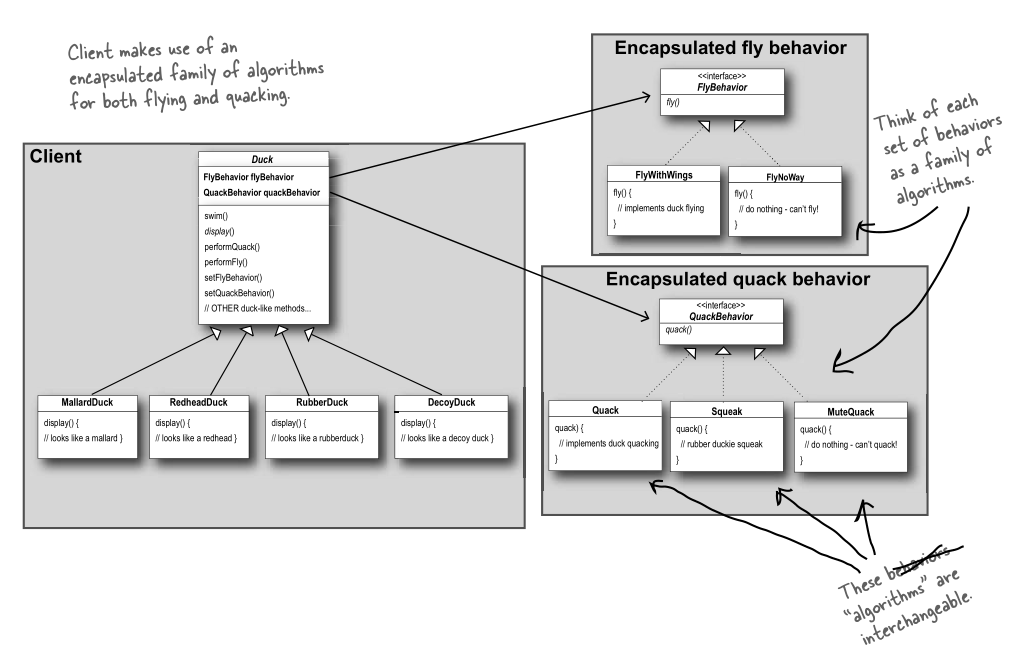
\includegraphics[width=\linewidth]{strategy/img/strategyUML}
	\caption{UML-Darstellung des Strategy-Musters}
	\label{fig:strategyUML}
\end{figure}